\documentclass[12pt,a4paper,dvipdf]{jsarticle}
\usepackage{listings}
\usepackage{amsmath, xparse}
\usepackage{xcolor}
\usepackage[dvipdfmx]{graphicx}
\usepackage{float}
\setlength{\textwidth}{\textwidth}
\setlength{\topmargin}{0pt}
\setlength{\headheight}{0pt}
\setlength{\headsep}{0pt}
\lstset{
    basicstyle = {\ttfamily}, % 基本的なフォントスタイル
    frame = {tbrl}, % 枠線の枠線。t: top, b: bottom, r: right, l: left
    breaklines = true, % 長い行の改行
    numbers = left, % 行番号の表示。left, right, none
    showspaces = false, % スペースの表示
    showstringspaces = false, % 文字列中のスペースの表示
    showtabs = false, % タブの表示
    keywordstyle = \color{blue}, % キーワードのスタイル。intやwhileなど
    commentstyle = {\color[HTML]{1AB91A}}, % コメントのスタイル
    identifierstyle = \color{black}, % 識別子のスタイル 関数名や変数名
    stringstyle = \color{brown}, % 文字列のスタイル
    captionpos = t % キャプションの位置 t: 上、b: 下
}
\title{簡易プロトタイピングによる\\ユーザインタフェース設計\\検討会説明用資料}
\author{202210779 山田 悠真\\202211879 新井 皓陽\\202212115 近 和}
\date{\today}
\begin{document}
\maketitle
\newpage
% \section{sample}
% \begin{figure}[H]
%     \centering
%     \includegraphics[width=10cm]{sample.png}
%     \caption{sample.png}
%     \label{fig:sample}
% \end{figure}


\section{制作するユーザーインターフェースの概要}
\subsection{制作するシステムを選定した経緯}
この実験では「空き教室確認システム」と題して教室の空き状況と設備情報を確認するシステムを作成した。対象システム制定の経緯としては、現在存在する学内マップや授業管理システムでは教室に着目したユーザーインターフェースがなく、教室ごとの利用状況を把握することが困難であるという問題があった。そのため、空き教室を確認するためのユーザーインターフェースを作成することを目標とした。また、キャンパスマップには学内マップに教室ごとの設備情報が掲載されているが、表形式で纏められているため教室の位置を把握することが困難である。故に、教室の設備情報を教室の位置情報と関連付けたユーザーインターフェースを作成することを目標とした。
\subsection{実験参加者に課す課題内容}
実験を行っていく間に発生した問題点を踏まえて逐次実験の手順を改善したため、最初の実験参加者に行った指示と異なる部分がある。
\subsubsection{「現在自分がいる建物内にある暗幕のある空き教室を見つけ、その教室番号を答える」}
この課題では、実験参加者は予め説明を受けた現在地マーカーを頼りに現在の自分が居る建物を確認する。その後、実験参加者は建物内マップのアイコンを頼りに階層を移動し、暗幕がある空き教室を把握することを想定している。また、この課題では、馴染みのあるエリアと馴染みのないエリアでの操作の差異を確認するため、現在地を3C棟に配置した場合と6A棟に配置した場合をシミュレーションした。
\begin{itemize}
    \item 縁取りされた教室が空き教室である(既知)
    \item 現在地はマップ上で現在地マーカーを用いて表される
    \item マップ上には教室名とともに利用可能な設備を示すアイコンが配置されている。
\end{itemize}

\subsubsection{「以下の条件をすべて満たす教室の教室番号を答える」}
この課題では、実験参加者は絞り込みの機能を用いて条件に適合する教室を把握し、その教室番号を答えることを想定している。\\
課す条件は以下の通りである。
\begin{itemize}
    \item 液晶プロジェクターが利用可能
    \item 3C棟内にある
    \item 1月31日 金曜日の15時15分から18時に利用可能である
    \item 収容人数が20人以上である
\end{itemize}

\subsubsection{「検索窓を用いて6A202ビジュアルデザイン室および3C113計算機室の利用予定表を確認する」}
この課題では、実験参加者は検索窓を用いて対象教室のの利用予定表を確認することを想定している。そのため、実験参加者には必ず検索窓を用いる旨を周知する。また、課題の対象となる教室については課題1と同様の理由で複数の教室を挙げているが、実験時間の都合で実験参加者にはそれぞれ片方の教室のみについて行ってもらった。
\begin{itemize}
    \item 実験参加者には検索窓を必ず用いる旨を周知する
    \item 検索窓には教室名を入力することのみを想定する
    \item 検索窓に途中まで入力した場合も予測して検索結果を出力する
\end{itemize}
\subsubsection{実験参加者に事前に周知する点}
\begin{itemize}
    \item 作成したシステムは筑波大学の空き教室を調べるサービスのシステムである
    \item 赤色に縁取られた教室は空き教室である
    \item 画面上部のアイコンから「エリア選択」、「キーワード検索」、「絞り込み検索」が行える
    \item 付箋をタップで文字を入力できる
    \item 課題は1から順に行う
    \item 各課題の開始時には大学全域地図の画面に初期化する
    \item 全課題終了後にアンケートがある
    \item 不明な点があれば課題開始前に口頭で質問を受け付ける
\end{itemize}

\newpage
\section{作成する画面のリストアップ}
\begin{enumerate}
    \item 全学エリアの地図
    \item 第123エリアの地図
    \item 第3エリアの地図
    \item 大学会館・体育・芸術エリアの地図
    \item 3C棟1階の地図
    \item 3C棟2階の地図
    \item 3C棟3階の地図
    \item 3C棟4階の地図
    \item 6A棟1階の地図
    \item 6A棟2階の地図
    \item 6A棟3階の地図
    \item 6A棟4階の地図
    \item 3C113の設備情報と利用予定表
    \item 6A202の設備情報と利用予定表
    \item 検索窓
    \item 検索画面
    \item 絞り込みタブ
    \item エリア選択タブ
    \item 絞り込み結果
\end{enumerate}

\newpage
\section{作成する画面のデザイン}
\begin{enumerate}
    \item 全学エリアの地図
    \item エリアの地図
    \item 棟の地図
    \item 教室の情報と利用予定表
    \item 検索
    \item エリア選択
    \item 絞り込み
    \item 絞り込み中の地図
\end{enumerate}
\begin{figure}[H]
    \centering
    \begin{minipage}[b]{0.24\columnwidth}
        \centering
        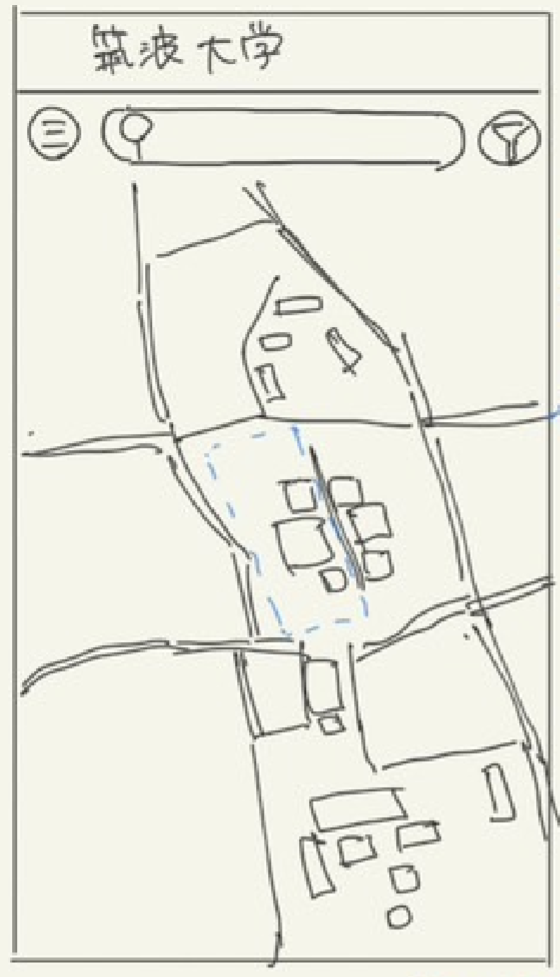
\includegraphics[width=0.9\columnwidth]{./img/全学地図.png}
        \caption{全学地図}
        \label{fig:全学地図}
    \end{minipage}
    \begin{minipage}[b]{0.24\columnwidth}
        \centering
        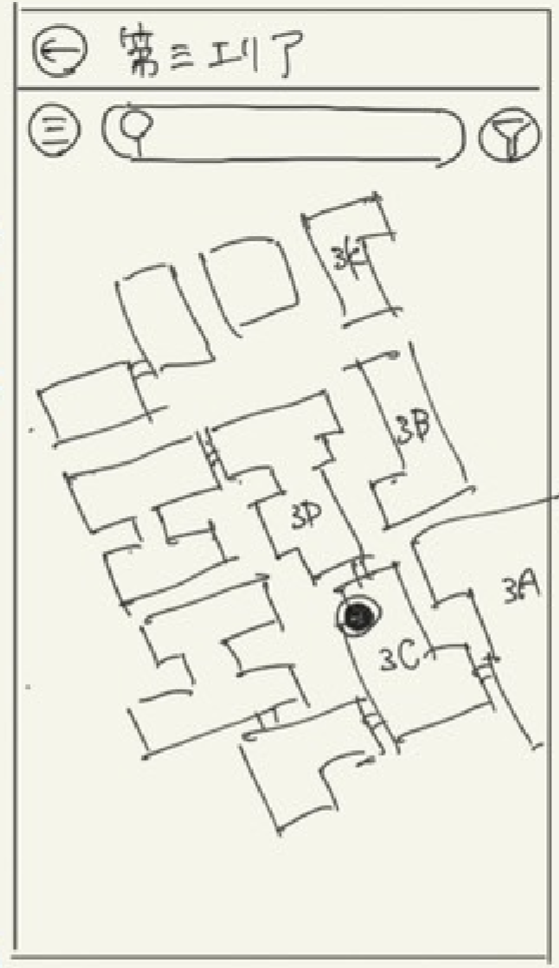
\includegraphics[width=0.9\columnwidth]{./img/エリア地図.png}
        \caption{エリア地図}
        \label{fig:エリア地図}
    \end{minipage}
    \begin{minipage}[b]{0.24\columnwidth}
        \centering
        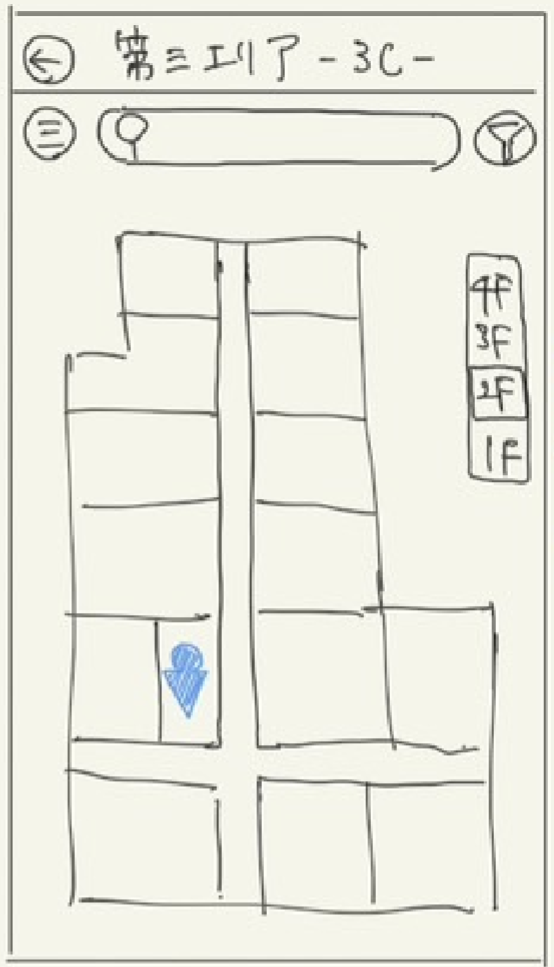
\includegraphics[width=0.9\columnwidth]{./img/棟地図.png}
        \caption{棟地図}
        \label{fig:棟地図}
    \end{minipage}
    \begin{minipage}[b]{0.24\columnwidth}
        \centering
        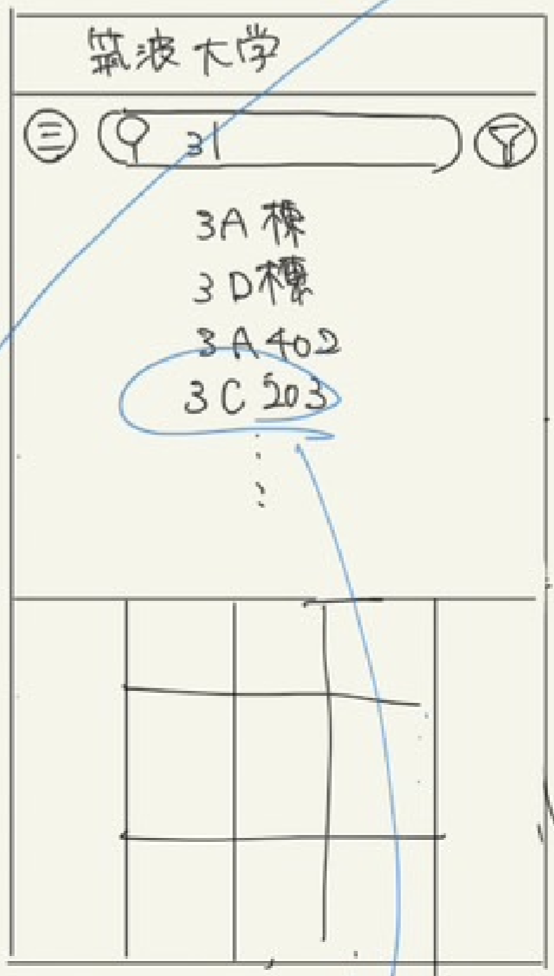
\includegraphics[width=0.9\columnwidth]{./img/検索.png}
        \caption{検索}
    \end{minipage}
\end{figure}
\begin{figure}[H]
    \centering
    \begin{minipage}[b]{0.24\columnwidth}
        \centering
        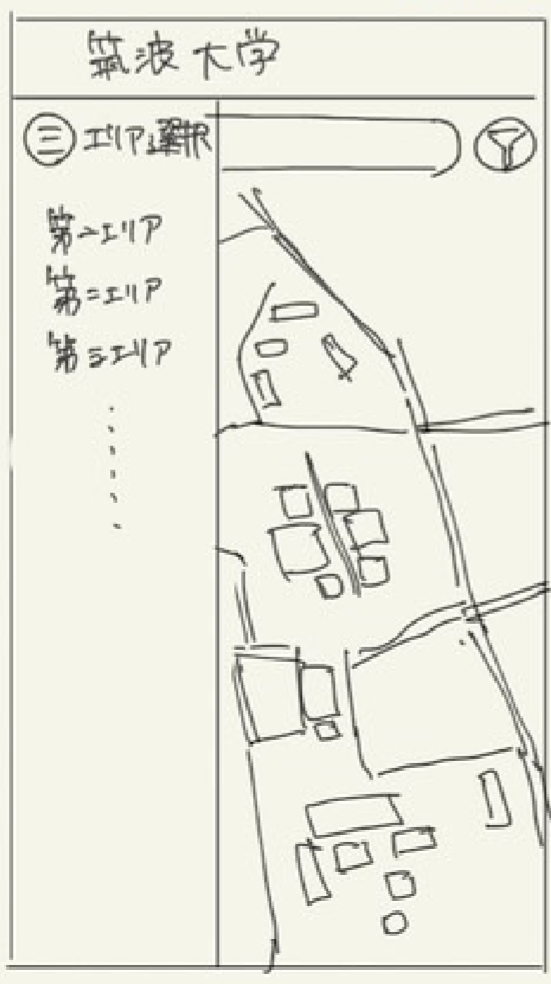
\includegraphics[width=0.9\columnwidth]{./img/エリア選択.png}
        \caption{エリア選択}
    \end{minipage}
    \begin{minipage}[b]{0.24\columnwidth}
        \centering
        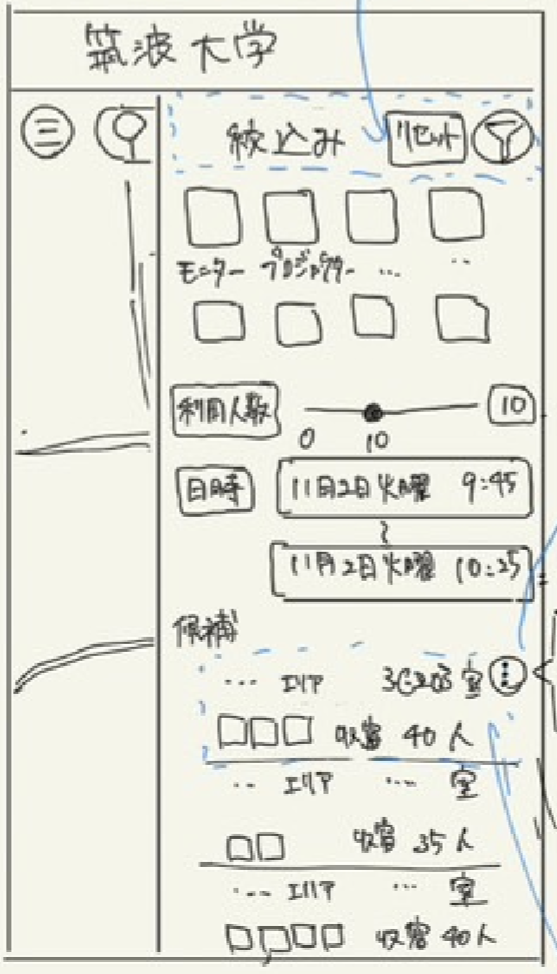
\includegraphics[width=0.9\columnwidth]{./img/絞り込み.png}
        \caption{絞り込み}
    \end{minipage}
    \begin{minipage}[b]{0.24\columnwidth}
        \centering
        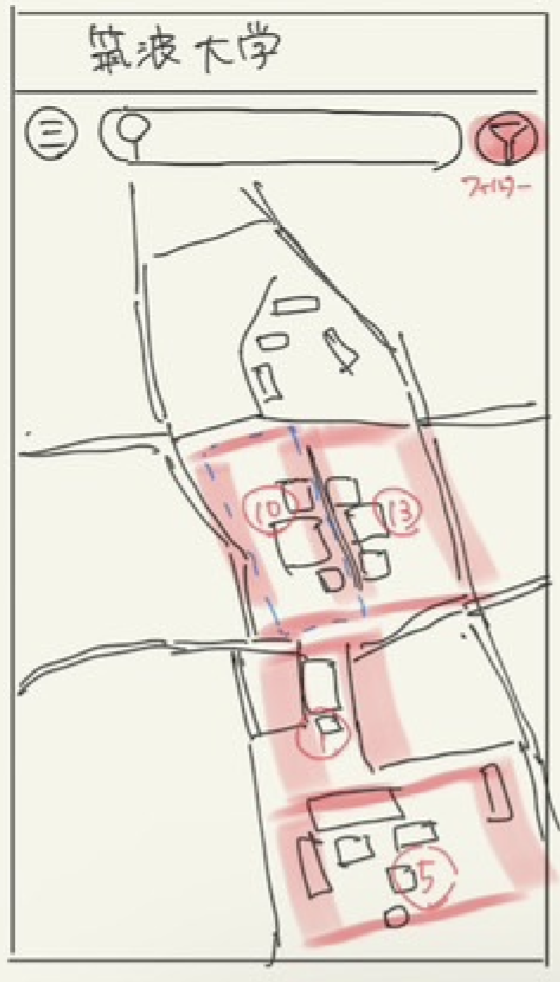
\includegraphics[width=0.9\columnwidth]{./img/絞り込み中.png}
        \caption{絞り込み中}
    \end{minipage}
    \begin{minipage}[b]{0.24\columnwidth}
        \centering
        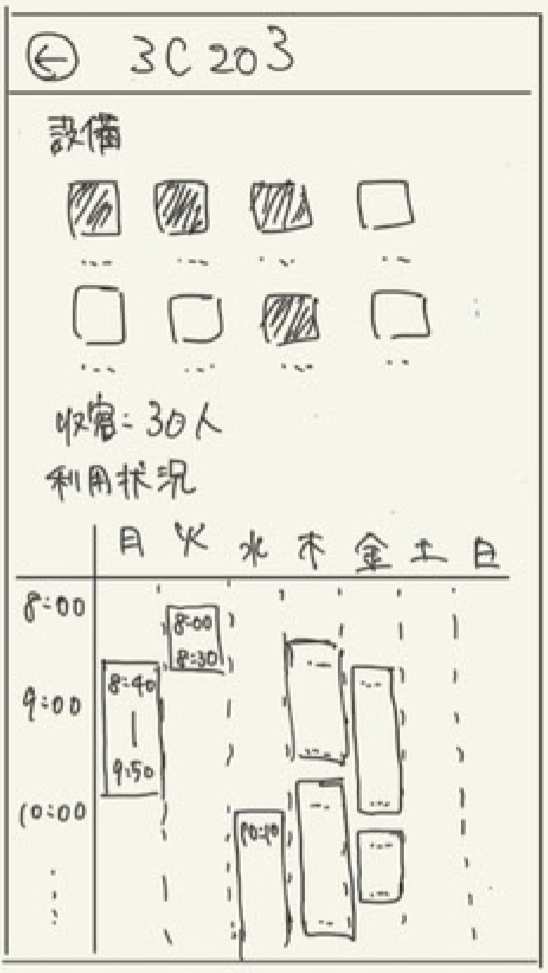
\includegraphics[width=0.9\columnwidth]{./img/部屋情報.png}
        \caption{部屋情報}
    \end{minipage}
\end{figure}



\newpage
\section{ユーザビリティテスト}
\subsection{取得データと取得方法}
\subsection{データの解析方法}
\subsection{データ解析の結果}
\subsubsection{想定したユーザー行動との相違}
\begin{itemize}
    \item
\end{itemize}
\subsubsection{問題点}
\begin{itemize}
    \item
\end{itemize}
\subsubsection{プロトタイプの修正}































\end{document}